\graphicspath{{./},{./intro_figs}}
\section{\texorpdfstring{\MakeUppercase{introduction}}{introduction}}
\label{sec:intro}

\counterwithin{figure}{section}

\subsection{The Swarm -- Components of an Active Galactic Nucleus}

Galactic nuclei are typically composed of a supermassive black hole (SMBH) and a nuclear star cluster \citep[NSC,][]{Ghez+98,Ghez+08}.
NSCs are the most massive type of star clusters \citep{Neumayer+20} with mean stellar densities typically $\sim10^2-10^6\,\Msun ~\text{pc}^{-3}$ \citep{GeorgievBoker14}.
Additionally, there are potentially 20,000 stellar mass black holes (BH) within the central parsec of the SMBH \citep{MiraldaGould00,Freitag+06} supported by observations and modeling of low-mass X-ray binaries in the Galactic center \citep{Hailey+18,Generozov+18}.
When gas accretes onto the SMBH from a dusty toroidal reservoir, it forms an accretion disk that can reach 1 to 10 pc in size turning the system into an active galactic nucleus (AGN).
This system can radiate at high luminosities across the electromagnetic (EM) spectrum \citep{Hubeny+01}.
The radiation from the broad line region (BLR) in the rapidly moving accretion disk and narrow line region (NLR) associated with clouds of slowly moving gas in its vicinity produce broad and narrow spectral features, respectively.
Their presence or omission from AGN spectra are thought to be the result of viewing angle effects and accretion rate \citep{Antonucci93,Netzer15} that obscure or permit their observation.
The SMBH is enveloped in a hot X-ray corona that bathes the disk in a time-varying radiation field.
Reverberation mapping utilizes the time-delayed reflecting and reprocessing of this radiation to study disk structure \citep{BlandfordMcKee82,Cackett+21,Secunda+24}.
Fast-spinning SMBH with strongly magnetized disks can produce jets that eject material with enough kinetic energy to leave the galaxy or galaxy cluster entirely \citep{Oei+24}.
The cartoon in \Fig{fig:agn-components} \citep{Thorne22} presents a schematic view of the environment.

\begin{figure}
\centering
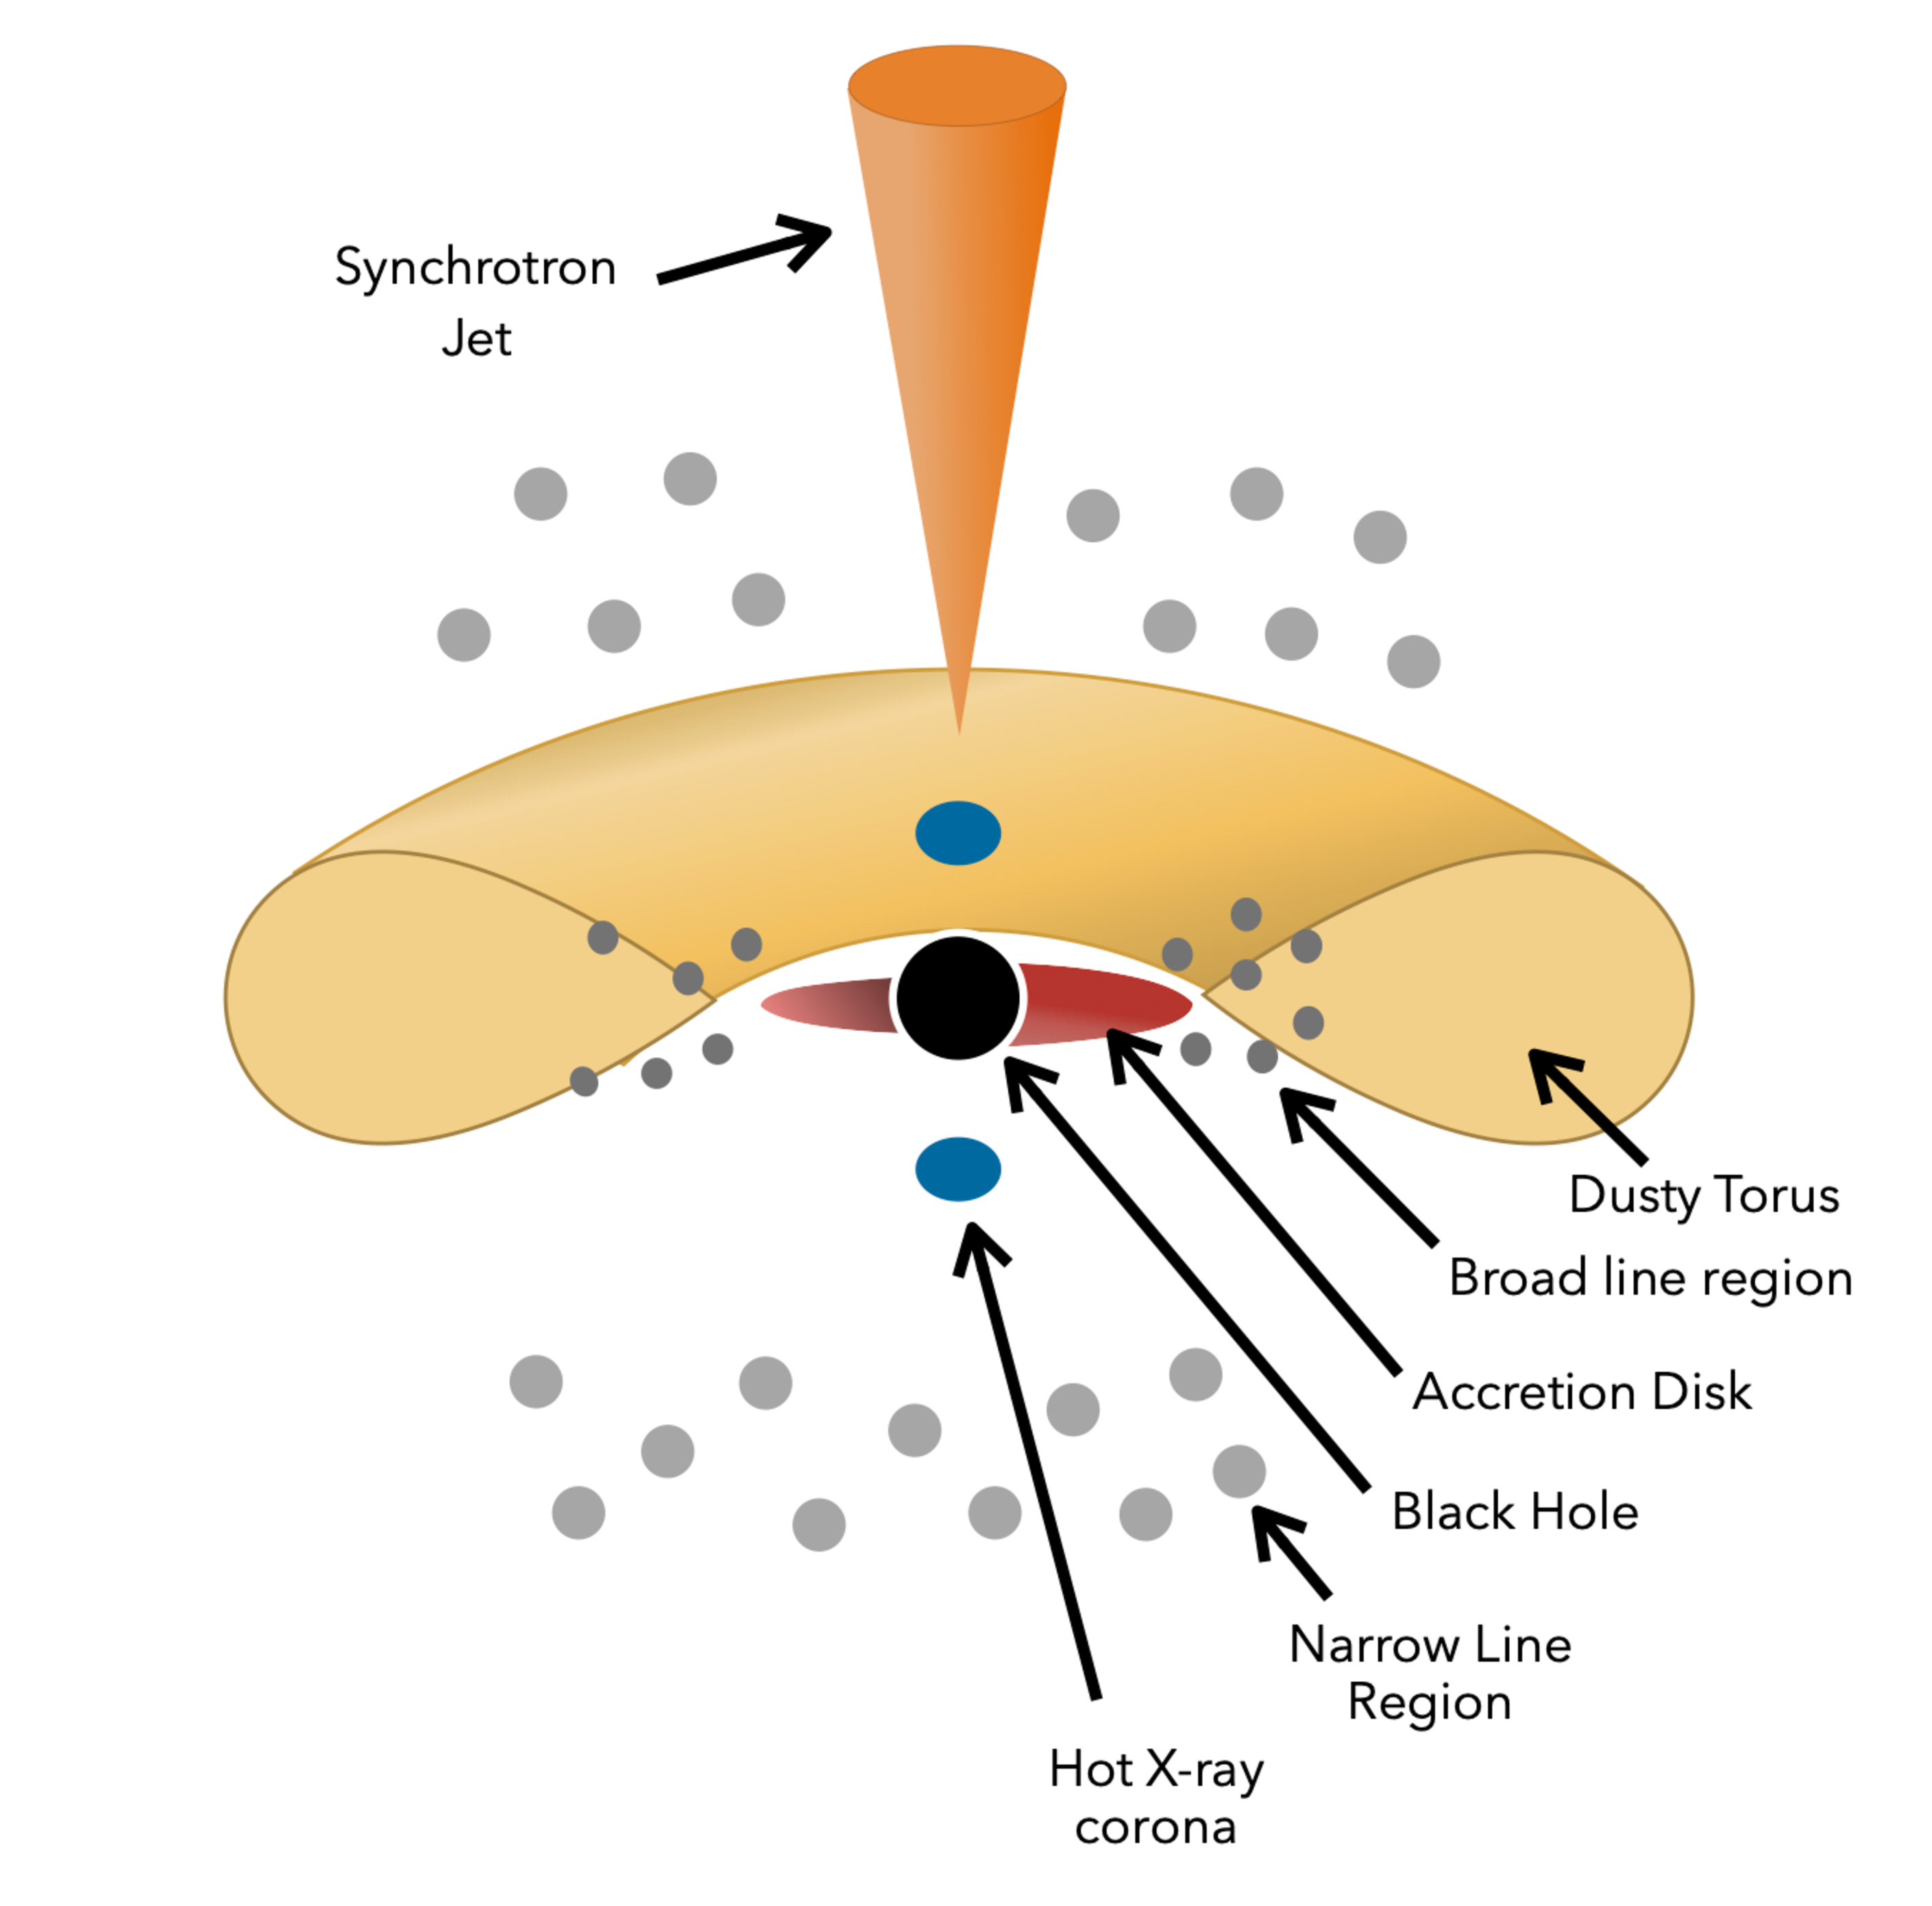
\includegraphics[width=1\textwidth]{intro_figs/AGNUnificationSteps_AGNComponents.pdf}
\caption[Components of an Active Galactic Nucleus]{Cartoon showing the various components of and AGN that affect observations.
The SMBH, accretion disk, and NSC (not shown) are of primary importance here.
Image credit: \citet{Thorne22}.}
\label{fig:agn-components}
\end{figure}



With such a high density of stars and BH in the vicinity of the SMBH, a fraction of the orbits will be embedded in the accretion disk, while others will have disk-crossing orbits.
Furthermore, AGN disks can quickly capture stars from the inclined population \citep{Fabj+20,MacLeodLin20}.
In addition to those stars initially embedded in the disk when it forms, self-gravitating AGN disks can naturally fragment and form new stars, particularly at large radii \citep{ShlosmanBegelman89, CollinZahn08}, though magnetic fields \citep{Gerling-Dunsmore+25, Tsung+25} and feedback from embedded objects \citep{HanklaJiangArmitage20} may inhibit collapse.
A hypothesis has been suggested that the disk may generate chains of hierarchical mergers between stellar-mass black holes that produce intermediate-mass black hole (IMBH) remnants \citep{McKernan+12,McKernan+14, Bartos+17, Stone+17, FordMcKernan25, Abbott+20-GW190521, LVK+25-GW231123}, much like the collisional growth model for planet formation in circumstellar disks \citep{Pollack+96}.
\Fig{fig:sbhcapture} shows a cartoon of this scenario.

\begin{figure}
\centering
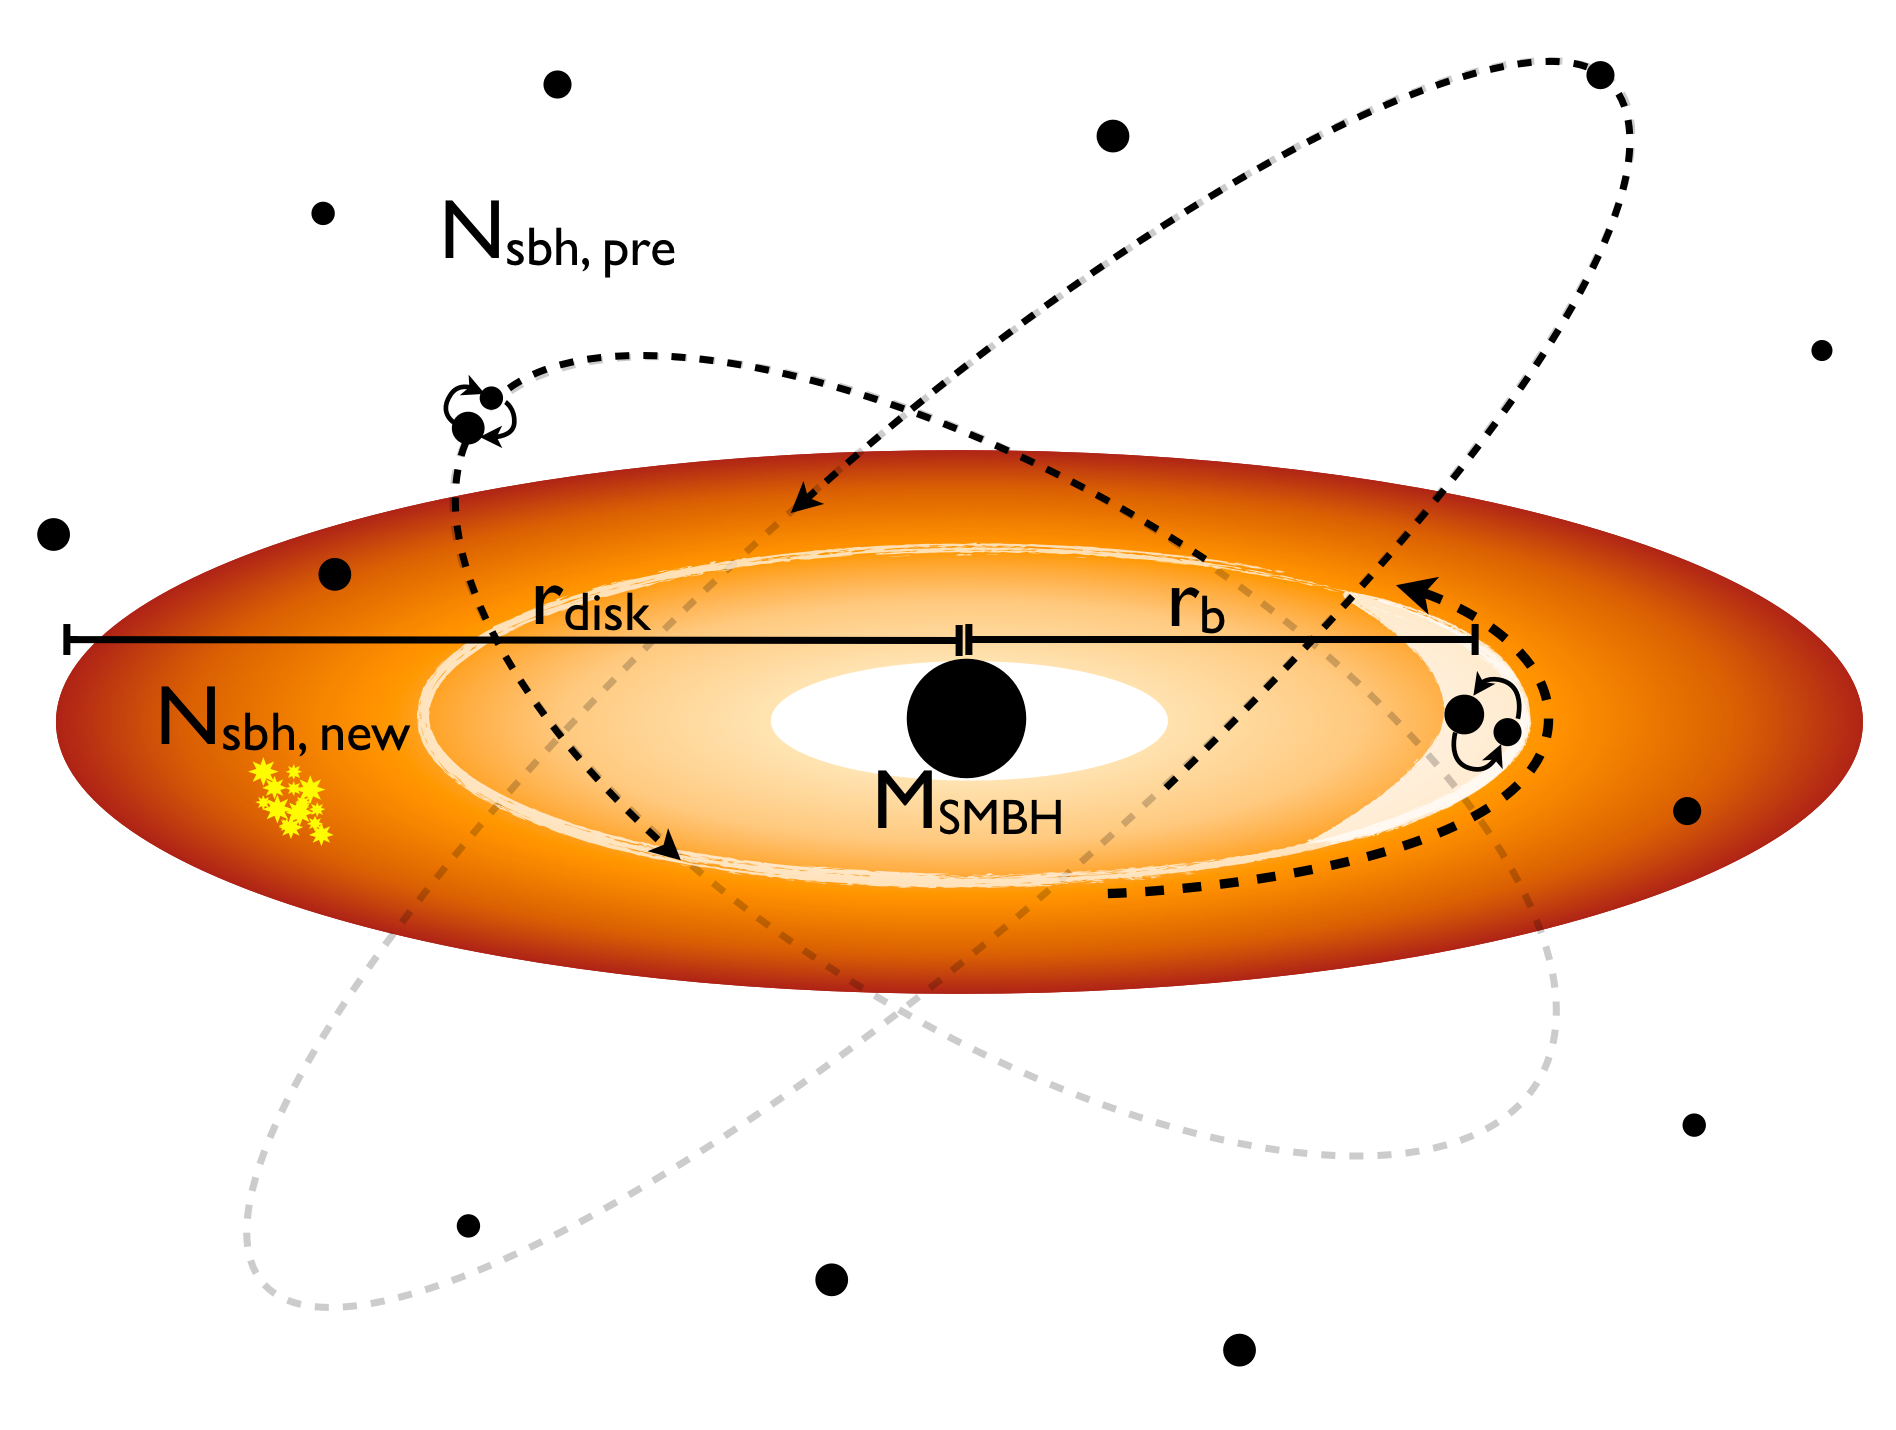
\includegraphics[width=1\textwidth]{intro_figs/sbhcapture2.png}
\caption[Interactions between an AGN disk and NSC]{Cartoon showing an AGN disk capturing BHs, forming binaries, and star formation.
Image credit: \citet{Ford+19}.}
\label{fig:sbhcapture}
\end{figure}


\subsection{The Sirens -- Multi-Messenger Probes of AGN Disks}
\subsubsection{Gravitational Waves}
Prior to 2015 the field of multi-messenger astronomy was restricted to three sources: EM radiation, cosmic rays, and neutrinos.
But on the 14th of September 2015, the first gravitational wave (GW) detection was made (called GW150914) by the Laser Interferometer Gravitational-Wave Observatory (LIGO) that was caused by the merging of two stellar mass black holes with masses $M=35_{-3}^{+5}\,\Msun$ and $30_{-4}^{+4}\,\Msun$ in the source frame \citep{GW150914}.
Two years later the first merger between two neutron stars (NS) was detected on the 17th of August 2017 \citep[GW170817,][]{nsGW170817}.
Though unknown at the time of detection, since the progenitor objects were not BHs, it was possible for the merger event to emit other forms of radiation.
The first such detection was gamma ray burst (GRB) named GRB 170817A observed by \emph{Fermi} and \emph{INTEGRAL}.
Then, an EM counterpart, named kilonova AT2017gfo, was observed in the galaxy NGC 4993 \citep{emGW170817} sparking a new age of multi-messenger astronomy.


\begin{figure}
\centering
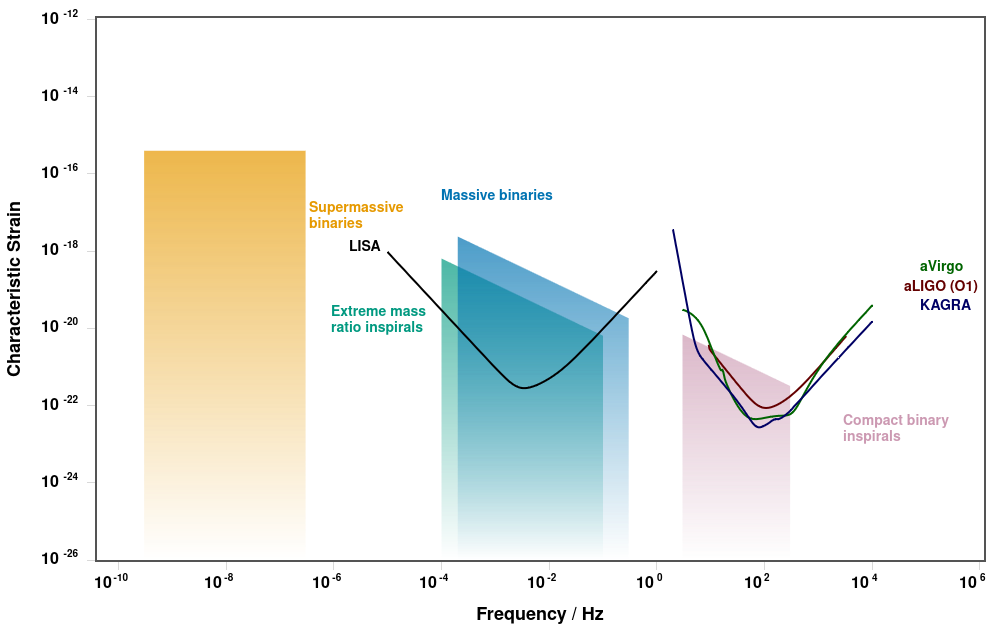
\includegraphics[width=1\linewidth]{intro_figs/gw-spectrum-detectors.png}
\caption[Gravitational wave source spectrum]{Categories of gravitational wave emitters and detector limits for LISA, aLIGO, aVirgo, and KAGRA.
Image credit: gwplotter.com \citep{Moore+15}.}
\label{fig:gwspectrum}
\end{figure}

LIGO and sister detectors Virgo and the Kamioka Gravitational Wave Detector (KAGRA) measure gravitational waves in the $\sim10-100$~Hz range that covers the final few moments of compact binary inspirals (see \Fig{fig:gwspectrum} that shows GW sources and detector limits).
In the future, the Laser Interferometer Space Antenna \citep[LISA,][]{LISA17,LISA23} will enable observations of extreme-mass ratio inspirals (EMRIs) and intermediate-mass ratio inspirals \citep[IMRIs,][]{Speri+26}.
These GW sources are comprised of single stellar mass BHs that emit long-lived GWs as they approach the event horizon of a SMBH and emit in the $\sim10^{-4}-10^{-1}$~Hz range.

Binary black hole (BBH) mergers are observed at an increasing rate as LIGO-Virgo-KAGRA (LVK) improve detector sensitivities \citep[e.g.][ see also \footnote{https://gracedb.ligo.org/superevents/public/O4/}]{Abbott+20-GW190521astro}.
Observed BBH include BH with individual masses in the expected upper mass gap ($\sim 50-120M_{\odot}$) where BHs are not expected from stellar evolution \citep{Belcynzski+16,RenzoSmith24} due to the pulsational pair instability.
A natural explanation for such BHs is via a series of hierarchical mergers that may occur in a dynamical environment, such as globular clusters \citep{Rodriguez+18}, NSC \citep{Antonini&Rasio16,Hoang+18,Fragione+19} and AGN accretion disks \citep{McKernan+12,McKernan+14,Bartos+17,StoneMetzgerHaiman17, ArcaSedda23,FordMcKernan25}.
Among hierarchical merger models, AGN are notable for both the efficiency of BBH formation as well as for retaining most post-merger products since even strong kicks from mergers correspond to small orbital perturbations in such a deep potential well.
This hypothesis is supported by the possibility that GW231123 is consistent with a merger between fourth and third generation BHs through the AGN channel \citep{Delfavero+25-GW231123}.

\subsubsection{Forming Binary Black Holes in Active Galactic Nuclear Accretion Disks}
Action of gas as a dynamical coolant and dynamical encounters drive BBH formation \citep[e.g.][]{Rowan+23,QianLiLai24,DodiciTremaine24}.
BHs embedded in AGN disks experience gas torques and can migrate \citep[e.g.][]{Syer+91,Levin07,McKernan+12}, where differential migration between BHs of different mass leads to encounters with other BH (as well as neutron stars and stars) and binary formation.
Binaries in AGN can be hardened or softened via dynamical encounters \citep[e.g.][]{Leigh+18,Samsing+20,Wang+21} or gas torques  \citep[e.g.][]{Tiede+20,Derdzinski+21,YapingLi+21}, resulting in a high rate of IMBH formation relative to other channels \citep{McKernan+12,Bellovary+16,Secunda+21,Yang+19,McKernan+20a,TagawaHaimanKocsis20,Vaccaro+24}.
Such mergers can occur at migration traps \citep[e.g.][]{Lyra+10,Sandor+11,Horn+12,Bellovary+16,Yang+19,Secunda+20}, in the bulk disk \citep[e.g.][]{Tagawa+20spin,McKernan+20a} and kicked outside the disk itself \citep{Tagawa+20b}.
However, if gap formation by IMBHs occurs, their presence may disrupt migration traps \citep{Gilbaum+25} but could also promote binary formation between nearby BHs through orbital resonances \citep{Horn+12} and at the gap edges \citep{KuchnerLecar02,Masset+06}.
The rate of BBH mergers from AGN is also expected to be significantly higher than from quiescent NSCs \citep{FordMcKernan22}.

These mergers in AGN disks should be detectable with gravitational waves \citep{McKernan+14,Bartos+17,Stone+17,Secunda+19} and could produce measurable EM counterparts from interactions with the AGN gas which would be otherwise absent for two black holes merging in the field \citep{McKernan+19,Perna+21}.

When BHs merge, we can retrieve the mass-weighted spin vector of the component BHs $\chi_i$ projected onto the binary's orbital angular momentum vector $\Lbin$ called the effective spin $\Xeff$.
This value ranges from -1 (both BH spins anti-aligned with $\Lbin$) to +1 (all vectors aligned; more about this in Ch.~\ref{sec:qXeff}, including a diagram shown in \Fig{fig:xeff-cartoon}).
The observed population of BBH mergers exhibits a bias towards $\Xeff>1$ \citep{Abbott+23-O3b}, implying they originate from formation channels that bias spin directions towards alignment with BBH orbital angular momentum.
This is not expected from gas-free hierarchical merger channels, but can occur in the AGN channel as BHs are torqued towards alignment with the gas disk over time \citep{Tagawa+20spin,Vajpeyi+22,McKernanFord24}.

Additionally, there is a possible anti-correlation observed in the mass ratio $q$ and effective spin $\Xeff$ distribution of BBH mergers \citep{Callister+21}.
This anit-correlation seems difficult to achieve in standard variants of other dynamical merger channels (e.g. globular clusters and NSC), although see \citet{Su25} for a discussion of how such an anti-correlation might arise in a dynamical triple channel.
In the isolated binary channel, \citet{Olejak+24,BanerjeeOlejak24} demonstrate the possibility of generating a $q$--$\Xeff$ anti-correlation via stable mass transfer.
In the AGN channel, an anti-correlation can arise due to several physical biases \citep{McKernan+22:q-Xeff,Santini+23, DittmannDempseyLi24}.
\citet{Vaccaro+24} show that if gas hardening is efficient in AGN, then the $q$--$\Xeff$ distribution should extend to significantly smaller values of $q$ and high $\Xeff$.
Thus, LVK O4 results can directly test gas hardening efficiency in AGN channel models, and through population studies, we can explore disk and NSC paramter space and binary formation mechanisms to give context for those GW observations.

Note that the AGN channel accounts for a still-uncertain fraction $f_{\rm AGN,BBH}$ of the observed LVK GW events.
We will learn considerably about the average properties of AGN and NSCs out to $z \sim 1$ by constraining $f_{\rm AGN, BBH}$, \emph{regardless of its actual value} (see \citealt{FordMcKernan25} for a more detailed discussion of this point).
Thus, in presenting distributions of AGN channel events in $q$--$\Xeff$ as a function of model choices, we are not claiming that AGN are responsible for all (or any) of the observed events.
Rather, we are demonstrating areas of AGN parameter space that might be ruled out by comparing with LVK O4 (O5) results that in turn hopefully allows us to constrain $f_{\rm AGN,BBH}$.




\subsubsection{Electromagnetic Waves}

As our detectors become more sensitive and the detection algorithms become more accurate, EM follow-up campaigns will become easier and more targeted.
Also, the expansion of transient surveys like the Legacy Survey through Space and Time (LSST) conducted by the Vera Rubin Telescope will allow archival searches for counterparts that could not be targeted in real time.
Yet, such a dynamic environment has the potential to produce many transient signals that must be distinguishable from one another to ensure we accurately identify counterparts to GW sources.
Among these are phenomena known as quasi-periodic oscillations (QPOs), quasi-periodic eruptions (QPEs), tidal disruption events (TDEs), changing-look AGN, supernovae (SNe) from the NSC, and anomalous flares.
These potential sources of noise must be studied to enable the search for potential EM counterparts to BBH mergers.

The first candidate EM counterpart to a gravitational wave detected binary black hole (BBH) merger was reportedly observed as a flare in AGN J124942.3+344929 by the Zwicky Transient Facility (ZTF) that was designated as ZTF19abanrhr \citep[][see \Fig{fig:counterpart-flare}]{Graham+20}.
Since the flare was inside the source volume of the gravitational wave detection GW190521 \citep{Abbott+20-GW190521} the authors suggest it could have been produced by the recoiling remnant black hole if the merger had occurred within the AGN accretion disk and experienced ram-pressure stripping of the gas bound within its Hill sphere by the disk \citep{McKernan+19}.
Using this model \citet{Graham+20} predicted a black hole mass $M\approx150\,\Msun$ which was later confirmed by the LIGO Scientific Collaboration and the Virgo Collaboration \citep{Abbott+20-GW190521}.

\begin{figure}
\centering
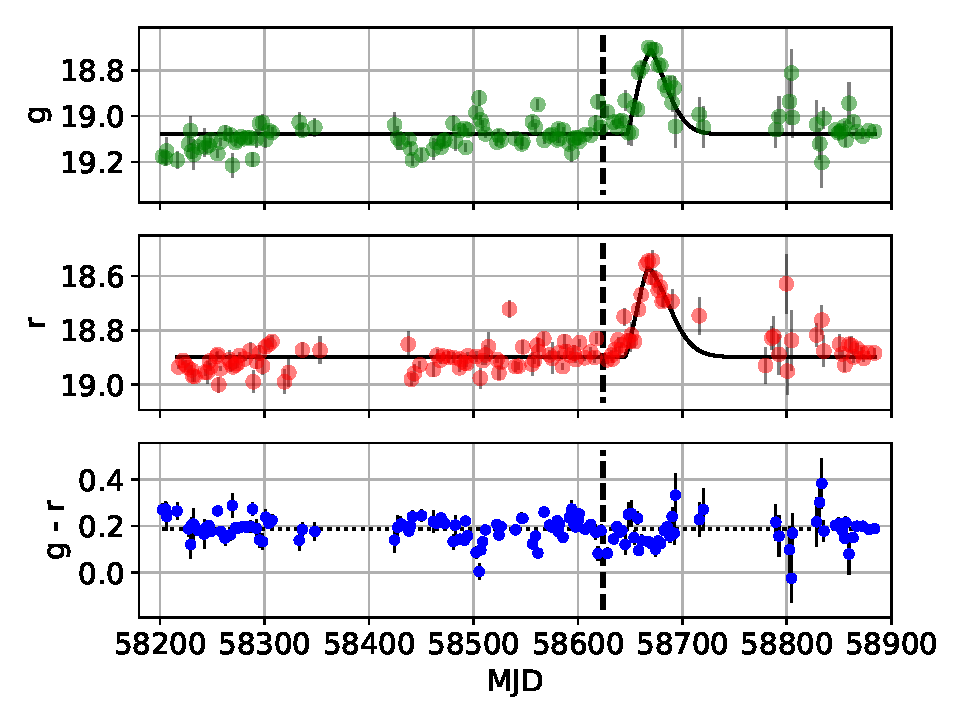
\includegraphics[width=1\textwidth]{intro_figs/counterpart-flare.pdf}
\caption[Proposed counterpart flare to GW190521]{ZTF $g$ and $r$ magnitudes and $g-r$ color for flare ZTF19abanrhr that has been proposed as an EM counterpart to GW190521 detected on the date marked by the dashed line.
Image credit: \citet{Graham+20}.}
\label{fig:counterpart-flare}
\end{figure}

They dismissed a SN as the source of the flare because it did not show any color evolution as is typical of SNe light curves \citep{Hueichapan+25}.
However, the integrated energy of the flare was $\sim10^{51}$ erg s$^{-1}$, which is conspicuously the typical energy budget of a core-collapse SN (or Type II).
A class of observed SNe are denoted as superluminous SNe (SLSNe) since their light curves peak above $\sim 10^{44}\,\text{erg s}^{-1}$ \citep{Gal-Yam12}.
One possible origin of these SLSNe is from stars that experienced extensive mass loss during their final years pre-SN \citep{Moriya+13}.
The amount of radiated energy increases with the envelope mass until the mass is similar to the ejecta mass, and the width of the light curve increases with the envelope size \citep{GinzburgBalberg12}.
If embedded SNe interact with a dense AGN disk in a similar way, their radiation may likely also be larger than their ``naked" cousins whereby the disk reprocesses much of their mechanical energy into radiation as the shock heats the disk, possibly making them observable against the bright AGN disk.
SNe in the dusty outskirts of AGN disks may have already been detected as bright optical and infrared flares \citep[e.g.][]{Assef+18}.

%We are motivated to explore the evolution of SNe embedded in an AGN disk due to the possibility that AGN flares could be EM counterparts to the gravitational wave detections from binary black hole (BBH) merger events, one particular case to underscore being GW190521 \citet{Abbott+20-GW190521}.
%While the observed flare \citep{Graham+20} did not resemble a standard SN light curve, embedded SNe could behave differently than SNe occurring in the ISM. 

%Galactic nuclei contain stars, some of which, if embedded in an active galactic nucleus (AGN) disk could detonate as embedded supernovae (SNe).
Any massive embedded stars may detonate as SNe within the disk confines, though stellar evolution in AGN disks may proceed very differently than in the interstellar medium \citep[ISM,][]{CantielloJermynLin21}.
Even in this case, SNe may yet result from stellar evolution \citep{Jermyn+21} or collisions and contribute to disk turbulence \citep{Moranchel+21}.

Whether the radiation from SNe escapes from an AGN disk is a separate matter from the mechanical breakout of the shockwave.
The non-uniform density and variable disk thickness have large impacts on a SN shock's morphological evolution in comparison to their galactic counterparts \citep{MacLowMcCray88}.
The right combination may slow down a SN shock significantly or prevent it from escaping entirely, thus depositing their kinetic energy in the disk.
These muffled SNe may not excavate the disk but could still be a contributing energy source for driving turbulence and maintaining pressure support in disks that would otherwise collapse under self-gravity \citep{Rozyczka+95,Moranchel+21}.

Characterizing light curves and color evolution from these embedded SNe is crucial for accurately distinguishing between potential transient events present in AGN disks during archival searches and live rapid-response follow-up campaigns for counterparts to gravitational wave events.
Furthermore, by understanding how SNe appear in AGN, we can rule out false positive counterparts to black hole mergers as well as constrain the rate of SNe in AGN.
Looking forward, detections of embedded SNe (or other transients in AGN disks) will allow us to constrain the composition, evolution, and dynamics of nuclear star clusters that coexist with an AGN disk, as well as to probe the disk properties.


\subsection{Primary Science Questions}

AGN are complex, dynamic systems that produce highly energetic events that impart large amounts of feedback on their environments.
It is possible that AGN disks are places to easily form and merge BBHs.
Since observing physical conditions in AGN disks and galactic nuclei in general is difficult, we can use population studies of GW detections from AGN with varying parameters to isolate parameters that reproduce the existing GW observations thereby constraining the physical conditions of the environment.
The presence of the gas provides a potential for EM counterparts to these mergers that would be impossible otherwise.
In order to accurately tie EM flares to BBH mergers, we must rule out other transients as potential sources of confusion.

\noindent To address these issues, we set out to investigate the following questions:

\begin{itemize}
\item \emph{Question 1:} What do the properties of binary black hole mergers in active galactic nucleus accretion disks reveal about the nuclear star cluster and disk properties?

\item \emph{Question 2:} What are the distinguishing characteristics of core-collapse supernovae that occur in accretion disks, and are they observable?
\end{itemize}




\subsection{Modeling Techniques}

We employ the following tools and methods to investigate the interactions between and the observational signatures of BBH mergers and SNe in AGN disks.

\subsubsection{Monte Carlo Simulations}

We use Monte Carlo simulations to explore the myriad process and vast parameter space involved with understanding how BBH form and merge in AGN disks.
Monte Carlo simulations are a numerical technique that randomly draws samples from a distribution of values that are assigned a probability of being selected.
Common probability distributions are uniform (the same probability everywhere) and Gaussian (with some characteristic mean and width), but they can be more sophisticated depending on the prior knowledge of the distribution being sampled.
Using this method, we draw random samples of parameters such as mass, orbital parameters, or spatial distributions to generate a representative subpopulation of quantities that evolve in time according to analytical expressions for physical processes.
This allows us to test different models for parameters and processes (e.g., accretion mechanism, orbital evolution, and mass functions) to compare their effects on the resulting merger population relative to each other.

The groundwork for this technique applied to mergers in AGN disks was laid out in \citet{McKernan+20a,McKernan+20b}.
The work presented details the effort to expand on it with a new code that is more robust, flexible, and user-friendly \citep{McKernan+25-mcfactsI,Cook+25,Delfavero+25-mcfactsIII,McPike+26-mcfactsIV}.

\subsubsection{Hydrodynamic Codes}

Hydrodynamics is the study of the physics of fluids.
For SNe embedded in AGN disks, the ejected material must expand into the dense disk.
Codes that solve the equations of hydrodynamics allow us to follow the strong shock interactions that occur between these two fluids.
\citet{Grishin+21} performed two-dimensional hydrodynamic simulations in the $r$-$z$ plane of SNe occurring in a flat slab of gas at the midplane and with a vertical offset, finding the shock breaks free from the disk above and below the midplane for both cases.
\citet{Moranchel+21} ran three-dimensional simulations in spherical coordinates for the upper half of the disk and find agreement that shocks from SNe at the midplane broke free from the disk.
We expand upon this work by estimating where SNe may break free from two AGN disk models using analytical expressions.
We verify these predictions with three-dimensional hydrodynamic simulations of a SN embedded in a vertically stratified shearing disk by exploring multiple radial and vertical locations in the disk with the \code{Athena} code \citep{Stone+08,StoneGardiner10}.

\subsubsection{Post-processing Radiative Transfer Methods}
Radiative transfer is one of the core tools at disposal to astronomers, since, until relatively recently, EM radiation was the sole mechanism by which to observe the Universe.
When properly considered, radiation can influence the temperature of a hydrodynamic system, so it would be best to include it as a component of the system of equations to solve for the hydrodynamic evolution.
However, solving radiation hydrodynamics in its full generality, by coupling the hydrodynamic equations with the equation of radiative transfer, is a formidable problem and computationally expensive, though some codes are making strides towards that end \citep[e.g.,][]{Jiang+14,White+23}.
An alternative is to apply post-processing radiative transfer algorithms to the output snapshots from a hydrodynamic code.

Existing codes were either proprietary \citep[\code{PHOENIX/3D},][]{Jack+09,HauschildtBaron10}, or we had difficulty modifying them to incorporate our hydrodynamic models \citep[\code{Sedona},][]{Kasen+06}.
We also looked into \code{RADMC-3D,} \citep{Dullemond+12-RADMC-3D}, which uses a Monte Carlo algorithm to solve the propagation of photon packets to converge on a temperature, but, there were concerns over whether it would converge in situations where non-thermodynamic equilibrium exist such as the AGN disk, SN ejecta, and nebular gas phases outside the disk.
We tried directly integrating the radiative transfer equation with AGN opacities, but that approach suffered from poor flux conservation.
We found instead that an implicit algorithm, the Feautrier method, afforded us greater accuracy, and developed our own code to implement this approach, that we called \ocotillo (we thank Shane Davis for suggesting this method).
\ocotillo simultaneously calculates the wavelength-dependent mean intensity, flux, and continuous opacity and applies it to the output from our SN models to retrieve integrated light curves and color evolutions.




We proceed to answer the questions posed above using these methods throughout the following chapters.

